\documentclass[11pt, compress]{beamer}
\usepackage{amsmath}
\usetheme{Boadilla}
\usefonttheme[onlymath]{serif}
%get rid of navigation:
\setbeamertemplate{navigation symbols}{}


 %%%% Start PreTeXt generated preamble: %%%%% 

%% Some aspects of the preamble are conditional,
%% the LaTeX engine is one such determinant
\usepackage{ifthen}
\newcommand{\tabularfont}{}
\usepackage[xparse, raster]{tcolorbox}
\tcbset{colback=white, colframe=white}
\NewTColorBox{image}{mmm}{boxrule=0.25pt, colframe=gray, left skip=#1\linewidth,width=#2\linewidth}
\RenewTColorBox{definition}{m}{colback=teal!30!white, colbacktitle=teal!30!white, coltitle=black, colframe=gray, boxrule=0.5pt, sharp corners=downhill, titlerule = 0.25pt, title={#1}}
\RenewTColorBox{theorem}{m}{colback=pink!30!white, colbacktitle=pink!30!white, coltitle=black, colframe=gray, boxrule=0.5pt, sharp corners=downhill, titlerule = 0.25pt, title={#1}}
\RenewTColorBox{proof}{}{boxrule=0.25pt, colframe=gray, colback=white, before upper={Proof:}, after upper={\qed}}
%% tcolorbox styles for sidebyside layout
\tcbset{ bwminimalstyle/.style={size=minimal, boxrule=-0.3pt, frame empty,
colback=white, colbacktitle=white, coltitle=black, opacityfill=0.0} }
\tcbset{ sbsstyle/.style={raster before skip=2.0ex, raster equal height=rows, raster force size=false} }
\tcbset{ sbspanelstyle/.style={bwminimalstyle} }
%% Enviroments for side-by-side and components
%% Necessary to use \NewTColorBox for boxes of the panels
%% "newfloat" environment to squash page-breaks within a single sidebyside
%% "xparse" environment for entire sidebyside
\NewDocumentEnvironment{sidebyside}{mmmm}
  {\begin{tcbraster}
    [sbsstyle,raster columns=#1,
    raster left skip=#2\linewidth,raster right skip=#3\linewidth,raster column skip=#4\linewidth]}
  {\end{tcbraster}}
%% "tcolorbox" environment for a panel of sidebyside
\NewTColorBox{sbspanel}{mO{top}}{sbspanelstyle,width=#1\linewidth,valign=#2}
%% For improved tables
\usepackage{array}
%% Some extra height on each row is desirable, especially with horizontal rules
%% Increment determined experimentally
\setlength{\extrarowheight}{0.2ex}
%% Define variable thickness horizontal rules, full and partial
%% Thicknesses are 0.03, 0.05, 0.08 in the  booktabs  package
\newcommand{\hrulethin}  {\noalign{\hrule height 0.04em}}
\newcommand{\hrulemedium}{\noalign{\hrule height 0.07em}}
\newcommand{\hrulethick} {\noalign{\hrule height 0.11em}}
%% We preserve a copy of the \setlength package before other
%% packages (extpfeil) get a chance to load packages that redefine it
\let\oldsetlength\setlength
\newlength{\Oldarrayrulewidth}
\newcommand{\crulethin}[1]%
{\noalign{\global\oldsetlength{\Oldarrayrulewidth}{\arrayrulewidth}}%
\noalign{\global\oldsetlength{\arrayrulewidth}{0.04em}}\cline{#1}%
\noalign{\global\oldsetlength{\arrayrulewidth}{\Oldarrayrulewidth}}}%
\newcommand{\crulemedium}[1]%
{\noalign{\global\oldsetlength{\Oldarrayrulewidth}{\arrayrulewidth}}%
\noalign{\global\oldsetlength{\arrayrulewidth}{0.07em}}\cline{#1}%
\noalign{\global\oldsetlength{\arrayrulewidth}{\Oldarrayrulewidth}}}
\newcommand{\crulethick}[1]%
{\noalign{\global\oldsetlength{\Oldarrayrulewidth}{\arrayrulewidth}}%
\noalign{\global\oldsetlength{\arrayrulewidth}{0.11em}}\cline{#1}%
\noalign{\global\oldsetlength{\arrayrulewidth}{\Oldarrayrulewidth}}}
%% Single letter column specifiers defined via array package
\newcolumntype{A}{!{\vrule width 0.04em}}
\newcolumntype{B}{!{\vrule width 0.07em}}
\newcolumntype{C}{!{\vrule width 0.11em}}
\newcommand{\lt}{<}
\newcommand{\gt}{>}
\newcommand{\amp}{&}

%% Begin: Semantic Macros
%% To preserve meaning in a LaTeX file
%%
%% \mono macro for content of "c", "cd", "tag", etc elements
%% Also used automatically in other constructions
%% Simply an alias for \texttt
%% Always defined, even if there is no need, or if a specific tt font is not loaded
\newcommand{\mono}[1]{\texttt{#1}}
%%
%% Following semantic macros are only defined here if their
%% use is required only in this specific document
%%
%% Used for inline definitions of terms
\newcommand{\terminology}[1]{\textbf{#1}}
%% End: Semantic Macros

\renewcommand{\d}{\displaystyle}
\newcommand{\N}{\mathbb N}
\newcommand{\B}{\mathbf B}
\newcommand{\Z}{\mathbb Z}
\newcommand{\Q}{\mathbb Q}
\newcommand{\R}{\mathbb R}
\def\C{\mathbb C}
\def\U{\mathcal U}
\newcommand{\pow}{\mathcal P}
\newcommand{\inv}{^{-1}}
\newcommand{\st}{:}
\renewcommand{\iff}{\leftrightarrow}
\newcommand{\Iff}{\Leftrightarrow}
\newcommand{\imp}{\rightarrow}
\newcommand{\Imp}{\Rightarrow}
\newcommand{\isom}{\cong}

\renewcommand{\bar}{\overline}
\newcommand{\card}[1]{\left| #1 \right|}
\newcommand{\twoline}[2]{\begin{pmatrix}#1 \\ #2 \end{pmatrix}}

\newcommand{\vtx}[2]{node[fill,circle,inner sep=0pt, minimum size=4pt,label=#1:#2]{}}
\newcommand{\va}[1]{\vtx{above}{#1}}
\newcommand{\vb}[1]{\vtx{below}{#1}}
\newcommand{\vr}[1]{\vtx{right}{#1}}
\newcommand{\vl}[1]{\vtx{left}{#1}}
\renewcommand{\v}{\vtx{above}{}}

%% Graphics Preamble Entries
\usepackage{tikz, pgfplots}

\usetikzlibrary{positioning,matrix,arrows}

\usetikzlibrary{shapes,decorations,shadows,fadings,patterns}
\usetikzlibrary{decorations.markings}

\usepackage{skak} %for chessboards etc.

\def\circleA{(-.5,0) circle (1)}
\def\circleAlabel{(-1.5,.6) node[above]{$A$}}
\def\circleB{(.5,0) circle (1)}
\def\circleBlabel{(1.5,.6) node[above]{$B$}}
\def\circleC{(0,-1) circle (1)}
\def\circleClabel{(.5,-2) node[right]{$C$}}
\def\twosetbox{(-2,-1.4) rectangle (2,1.4)}
\def\threesetbox{(-2.5,-2.4) rectangle (2.5,1.4)}
\newcommand{\hexbox}[3]{
  \def\x{-cos{30}*\r*#1+cos{30}*#2*\r*2}
  \def\y{-\r*#1-sin{30}*\r*#1}
  \draw (\x,\y) +(90:\r) -- +(30:\r) -- +(-30:\r) -- +(-90:\r) -- +(-150:\r) -- +(150:\r) -- cycle;
  \draw (\x,\y) node{#3};
}

\tikzset{->-/.style={decoration={
  markings,
  mark=at position .5 with {\arrow{>}}},postaction={decorate}}}

  \newcommand{\onedot}{
    +(.5,.5) \v
  }
  \newcommand{\twodots}{
    +(.25,.25) \v +(.75,.75) \v
  }
  \newcommand{\threedots}{
  +(.25,.25) \v +(.5, .5) \v +(.75,.75) \v
  }
  \newcommand{\fourdots}{
    +(.25,.25) \v +(.25,.75) \v +(.75,.25) \v +(.75,.75) \v
  }
  \newcommand{\fivedots}{
    +(.5,.5) \v +(.25,.25) \v +(.25,.75) \v +(.75,.25) \v +(.75,.75) \v
  }
  \newcommand{\sixdots}{
    +(.25,.5) \v +(.75,.5) \v +(.25,.25) \v +(.25,.75) \v +(.75,.25) \v +(.75,.75) \v
  }
  \newcommand{\dominoborder}{
    \draw[thick, rounded corners] (0,0) rectangle (1,2);
    \draw[thin] (0,1) -- (1,1);
  }


%%%% End of PreTeXt generated preamble %%%%% 

\title{Binomial Coefficients}
\subtitle{(Section 1.2)}
\author{}
\date[]{}

\begin{document}
\begin{frame}
\maketitle 
\end{frame}
 
\begin{frame}
\frametitle{Overview}
\tableofcontents 
\end{frame}
 

\section{Investigate}
\begin{frame}
\frametitle{Investigate!}
 In chess, a rook can move only in straight lines (not diagonally). Fill in each square of the chess board below with the number of different shortest paths the rook, in the upper left corner, can take to get to that square. For example, one square is already filled in. There are six different paths from the rook to the square: DDRR (down down right right), DRDR, DRRD, RDDR, RDRD and RRDD.
 \begin{sidebyside}{1}{0.25}{0.25}{0}%
\begin{sbspanel}{0.5}%
\resizebox{\linewidth}{!}{%
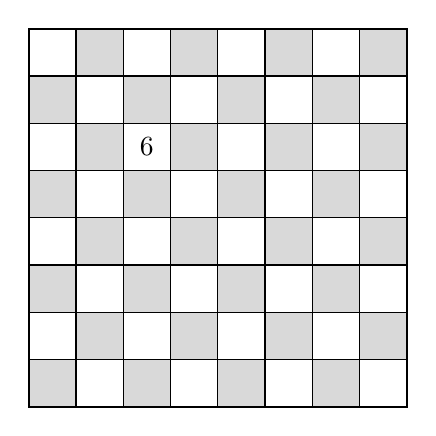
\begin{tikzpicture}[scale=.6]
\foreach \row in {0, 2, 4,6}{
  \foreach \col in {0,2,4,6}{
  \draw[fill=gray!30] (\row,\col) rectangle (\row+1, \col+1) rectangle (\row+2, \col+2);
  }
}
\draw[thick] (0,0) rectangle (8,8);
\node at (0.5,7.5) {\Large \symrook};
\node at (2.5,5.5) {$6$};
\end{tikzpicture}
}%
\end{sbspanel}%
\end{sidebyside}%
\end{frame}
 


\section{Subsets}
\begin{frame}
\frametitle{}
Let \(A = \{1,2,3,4,5\}\).  How many subsets are there of \(A\)?
 
\pause \vfill 

How many subsets of \(A\) have 3 elements?
 First, decide how many subsets have 0 elements, how many have 1 element, and how many have 4 or 5 elements.
 
\pause \vfill 

The number of subsets with 3 elements will be the same as the number of subsets with 2 elements.  How many are there?
\end{frame}
 
\begin{frame}
\frametitle{Number of subsets by cardinality}
 Let \(A = \{1,2,3,4,5\}\).  How many subsets are there of \(A\)?
 \begin{sidebyside}{1}{0}{0}{0}%
\begin{sbspanel}{1}%
{\centering%
{\tabularfont%
\begin{tabular}{lllllll}
\multicolumn{1}{c}{Number of elements:}&\multicolumn{1}{c}{0}&\multicolumn{1}{c}{1}&\multicolumn{1}{c}{2}&\multicolumn{1}{c}{3}&\multicolumn{1}{c}{4}&\multicolumn{1}{c}{5}\tabularnewline\hrulethin
\multicolumn{1}{c}{Number of subsets:}&\multicolumn{1}{c}{1}&\multicolumn{1}{c}{5}&\multicolumn{1}{c}{10}&\multicolumn{1}{c}{10}&\multicolumn{1}{c}{5}&\multicolumn{1}{c}{1}
\end{tabular}
}%
\par}
\end{sbspanel}%
\end{sidebyside}%
\end{frame}
 


\section{Bit Strings}
\begin{frame}
\frametitle{Bit Strings}
 ``Bit'' is short for ``binary digit,'' so a \terminology{bit string} is a string of binary digits. The \terminology{binary digits} are simply the numbers 0 and 1. All of the following are bit strings:%
\begin{equation*}
1001 \quad 0 \quad 1111 \quad 1010101010\text{.}
\end{equation*}

\end{frame}
 
\begin{frame}
\frametitle{Bit Strings}
 
\pause 

\begin{itemize}[<+->]
\item{} An \terminology{\(n\)-bit string} is a bit string of length \(n\). That is, it is a string containing \(n\) symbols, each of which is a bit, either 0 or 1.


\item{} The \terminology{weight} \index{weight, of a string} of a bit string is the number of 1's in it.


\item{} \(\B^n\) is the \emph{set} of all \(n\)-bit strings.

\item{} \(\B^n_k\) is the set of all \(n\)-bit strings of weight \(k\).
\end{itemize}

 
\pause \vfill 

For example, the elements of the set \(\B^3_2\) are the bit strings 011, 101, and 110. Those are the only strings containing three bits exactly two of which are 1's.
\end{frame}
 
\begin{frame}
\frametitle{Counting bit strings}
 The counting questions: How many bit strings have length 5? How many of those have weight 3? In other words, we are asking for the cardinalities \(|\B^5|\) and \(|\B^5_3|\).
 
\pause \vfill 

\(\card{\B^5} = 32\)
 
\pause \vfill 

\(\card{\B^5_3}\)... harder.
\end{frame}
 
\begin{frame}
\frametitle{A recurrence relation}
 Each string in \(\B^5_3\) starts with either a 0 or a 1.
 
\pause \vfill 

If it starts with a 0, the remaining bits form a string in \(\B^4_3\).
 If it starts with a 1, the remaining bits form a string in          \(\B^4_2\).
 
\pause \vfill 

Thus we have,%
\begin{equation*}
|\B^5_3| = |\B^4_2| + |\B^4_3|\text{.}
\end{equation*}
Now find \(|\B^5_3|\) (work backwards more if needed).
\end{frame}
 
\begin{frame}
\frametitle{32 and 10?}
 Our answers to the bit string questions were the same as the answers to the subsets question.  Why?
 
\pause \vfill 

Compare: \(11001\) to \(\{1, 2, 5\}\).
 Does \(01011\) correspond to a subset?
 Does \(\{2,3,4\}\) correspond to a bit sting?
\end{frame}
 


\section{Lattice Paths}
\begin{frame}
\frametitle{Lattice Paths}
 The \terminology{integer lattice} is the set of all points in the Cartesian plane for which both the \(x\) and \(y\) coordinates are integers.
 A \terminology{lattice path} is one of the shortest possible paths connecting two points on the lattice, moving only horizontally and vertically.
 For example, here are three possible lattice paths from the points \((0,0)\) to \((3,2)\):
 \begin{sidebyside}{3}{0.0166666666666667}{0.0166666666666667}{0.0333333333333333}%
\begin{sbspanel}{0.3}%
\resizebox{\linewidth}{!}{%
      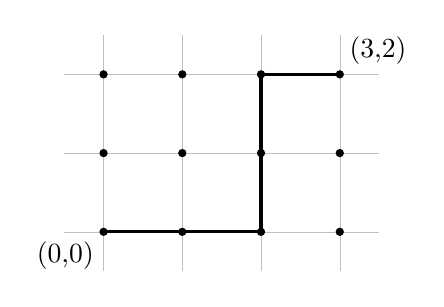
\begin{tikzpicture}
  \draw[very thin, color=gray!50] (-.5,-.5) grid (3.5, 2.5);
  \foreach \x in {0,...,3}
  \foreach \y in {0,...,2}
  \fill (\x,\y) circle (1.5pt);
  \draw (0,0) node[below left] { (0,0)} (3,2) node[above right] { (3,2)};
  \draw[very thick] (0,0) -- (2,0) -- (2,2) -- (3,2);
\end{tikzpicture}
}%
\end{sbspanel}%
\begin{sbspanel}{0.3}%
\resizebox{\linewidth}{!}{%
      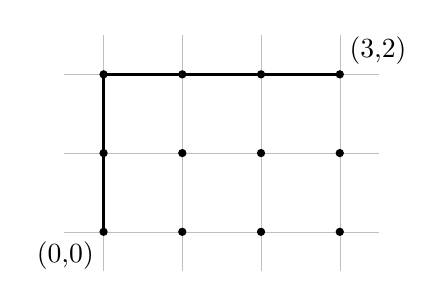
\begin{tikzpicture}
  \draw[very thin, color=gray!50] (-.5,-.5) grid (3.5, 2.5);
  \foreach \x in {0,...,3}
  \foreach \y in {0,...,2}
  \fill (\x,\y) circle (1.5pt);
  \draw (0,0) node[below left] { (0,0)} (3,2) node[above right] { (3,2)};
  \draw[very thick] (0,0) -- (0,2) -- (3,2);
\end{tikzpicture}
}%
\end{sbspanel}%
\begin{sbspanel}{0.3}%
\resizebox{\linewidth}{!}{%
      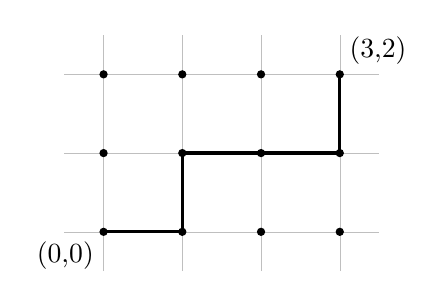
\begin{tikzpicture}
  \draw[very thin, color=gray!50] (-.5,-.5) grid (3.5, 2.5);
  \foreach \x in {0,...,3}
  \foreach \y in {0,...,2}
  \fill (\x,\y) circle (1.5pt);
  \draw (0,0) node[below left] { (0,0)} (3,2) node[above right] { (3,2)};
  \draw[very thick] (0,0) -- (1,0) -- (1,1) -- (3,1) -- (3,2);
\end{tikzpicture}
}%
\end{sbspanel}%
\end{sidebyside}%
\end{frame}
 
\begin{frame}
\frametitle{Counting Lattice Paths}
 The counting question: how many lattice paths are there between \((0,0)\) and \((3,2)\)?
 
\pause \vfill 

We could try to draw all of these, or instead of drawing them, maybe just list which direction we travel on each of the 5 steps.
 One path might be RRUUR, or maybe UURRR, or perhaps RURRU (those correspond to the three paths drawn above). So how many such strings of R's and U's are there?
\end{frame}
 
\begin{frame}
\frametitle{}
Here is another way to count lattice paths. Consider the lattice shown below:
 \begin{sidebyside}{1}{0.3}{0.3}{0}%
\begin{sbspanel}{0.4}%
\resizebox{\linewidth}{!}{%
      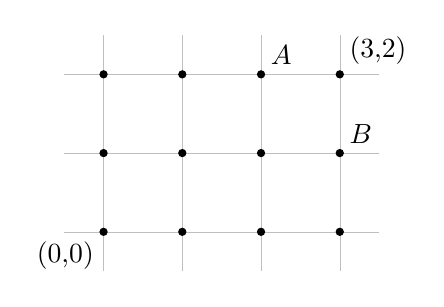
\begin{tikzpicture}
  \draw[very thin, color=gray!50] (-.5,-.5) grid (3.5, 2.5);
  \foreach \x in {0,...,3}
  \foreach \y in {0,...,2}
  \fill (\x,\y) circle (1.5pt);
  \draw (0,0) node[below left] { (0,0)} (3,2) node[above right] { (3,2)};
  \draw (3,1) node[above right] { \(B\)} (2,2) node[above right]{ \(A\)};
\end{tikzpicture}
}%
\end{sbspanel}%
\end{sidebyside}%
 Any lattice path from (0,0) to (3,2) must pass through exactly one of \(A\) and \(B\). The point \(A\) is 4 steps away from (0,0) and two of them are towards the right.
 
\pause \vfill 

The point: the exact same recurrence relation exists for bit strings and for lattice paths.
\end{frame}
 


\section{Binomial Coefficients}
\begin{frame}
\frametitle{Binomial Coefficients}
 \terminology{Binomial coefficients} are the coefficients in the expanded version of a binomial, such as \((x+y)^5\).
 
\pause \vfill 

What happens when we multiply such a binomial out? We will expand \((x+y)^n\) for various values of \(n\).%
\begin{equation*}
(x+y)^1 = x + y
\end{equation*}
%
\begin{equation*}
(x+y)^2 = x^2 + 2xy + y^2
\end{equation*}
%
\begin{equation*}
(x+y)^3 = x^3 + 3x^2y + 3xy^2 + y^3
\end{equation*}
%
\begin{equation*}
(x+y)^4 = x^4 + 4x^3y + 6x^2y^2 + 4xy^3 + y^4\text{.}
\end{equation*}

\end{frame}
 
\begin{frame}
\frametitle{}
There is a quicker way to expand these binomials. Consider the next one, \((x+y)^5\). What we are really doing is multiplying out,%
\begin{equation*}
(x+y)(x+y)(x+y)(x+y)(x+y)\text{.}
\end{equation*}

 
\pause \vfill 

Just find the coefficient of \(x^3y^2\). We must pick exactly 3 of the 5 binomials to contribute an \(x\), the other two to contribute a \(y\).
 
\pause \vfill 

We have 5 things, each can be one of two things, and we need a total of 3 of one of them. That's just like taking 5 bits and making sure exactly 3 of them are 1's. So the coefficient of \(x^3y^2\) (and also \(x^2y^3\)) will be exactly the same as the number of bit strings of length 5 and weight 3, which we found earlier to be 10.
 
\pause \vfill 

We have:%
\begin{equation*}
(x+y)^5 = x^5 + 5x^4y + 10x^3y^2 + 10x^2y^3 + 5 xy^4 + y^5\text{.}
\end{equation*}

\end{frame}
 
\begin{frame}
\frametitle{Binomial Coefficients}
 For each integer \(n \ge 0\) and integer \(k\) with \(0 \le k \le n\) there is a number%
\begin{equation*}
{n\choose k}\text{,}
\end{equation*}
read ``\(n\) choose \(k\).'' We have:\begin{itemize}
\item{} \({n\choose k} = |\B^n_k|\), the number of \(n\)-bit strings of weight \(k\).

\item{} \({n \choose k}\) is the number of subsets of a set of size \(n\) each with cardinality \(k\).

\item{} \({n \choose k}\) is the number of lattice paths of length \(n\) containing \(k\) steps to the right.

\item{} \({n \choose k}\) is the coefficient of \(x^ky^{n-k}\) in the expansion of \((x+y)^n\).

\item{} \({n \choose k}\) is the number of ways to select \(k\) objects from a total of \(n\) objects.
\end{itemize}

\end{frame}
 
\begin{frame}
\frametitle{Recurrence relation for \({n \choose k}\)}
 %
\begin{equation*}
{n \choose k} = {n-1 \choose k-1} + {n-1 \choose k}\text{.}
\end{equation*}

\end{frame}
 


\section{Pascal's Triangle}
\begin{frame}
\frametitle{}
\begin{sidebyside}{1}{0}{0}{0}%
\begin{sbspanel}{1}%
\resizebox{\linewidth}{!}{%
  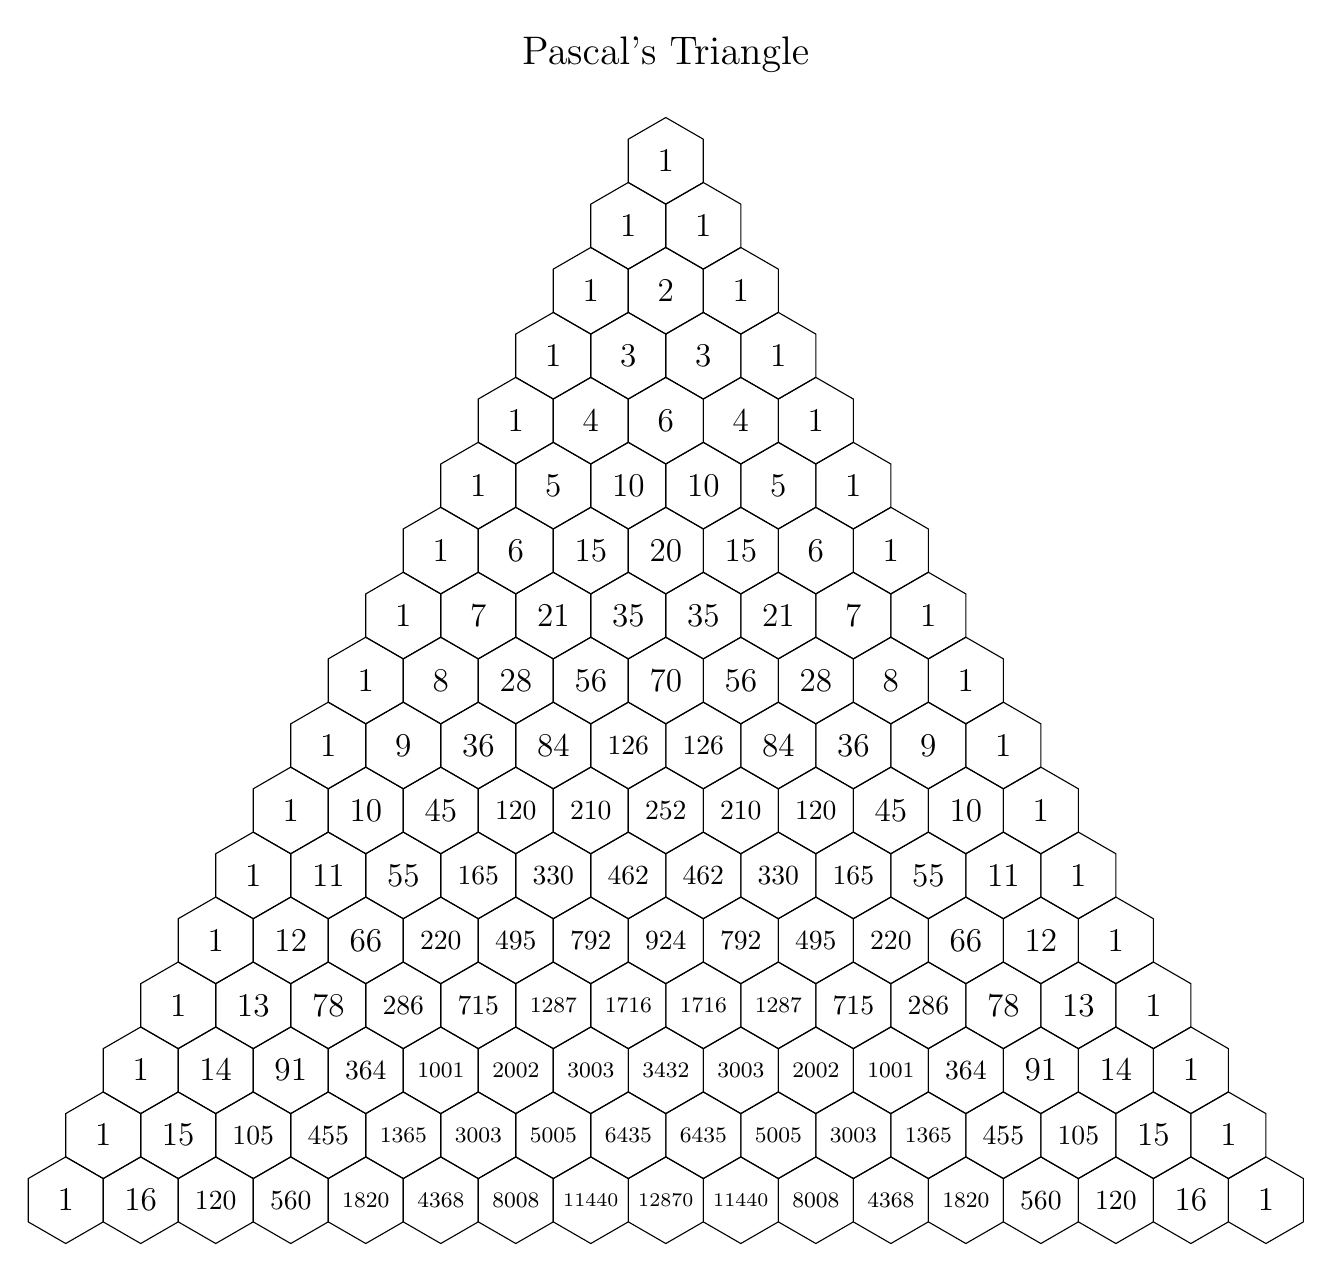
\begin{tikzpicture}
\def\r{.55}
\foreach \row in {0,...,16} {
  \hexbox{\row}{0}{\large 1}
}
%fill in the rest of the triangle:
\foreach \row in {1,...,16} {
  \pgfmathsetmacro{\entry}{1};
  \foreach \col in {1,...,\row} {
    % iterative formula : val = precval * (row-col+1)/col
    % (+ 0.5 to bypass rounding errors)
    \pgfmathtruncatemacro{\entry}{\entry*((\row-\col+1)/\col)+0.5}; \global\let\entry=\entry
    \ifnum \entry<100
\hexbox{\row}{\col}{\large \entry}
    \else \ifnum \entry<1000
\hexbox{\row}{\col}{\entry}
    \else \ifnum \entry<10000
\hexbox{\row}{\col}{\footnotesize \entry}
\else
\hexbox{\row}{\col}{\scriptsize \entry}
\fi
    \fi
    \fi
  }
}
\node[above] at (0,1) {\Large Pascal's Triangle};
\end{tikzpicture}
}%
\end{sbspanel}%
\end{sidebyside}%
\end{frame}
 

\end{document}
